\section*{Question 2}

\textit{ Plot the Probability Density Function (PDF) of the streamwise velocity gradient (i.e. $^{\partial u_1} / _{\partial x_1}$) from both datasets and calculate its first four moments. Using the moment information, comment on type of distribution exhibited by gradients in the two sets of data. Use Taylor’s hypothesis to convert temporal gradient to spatial gradient.}

\begin{figure}[!ht]
\centering
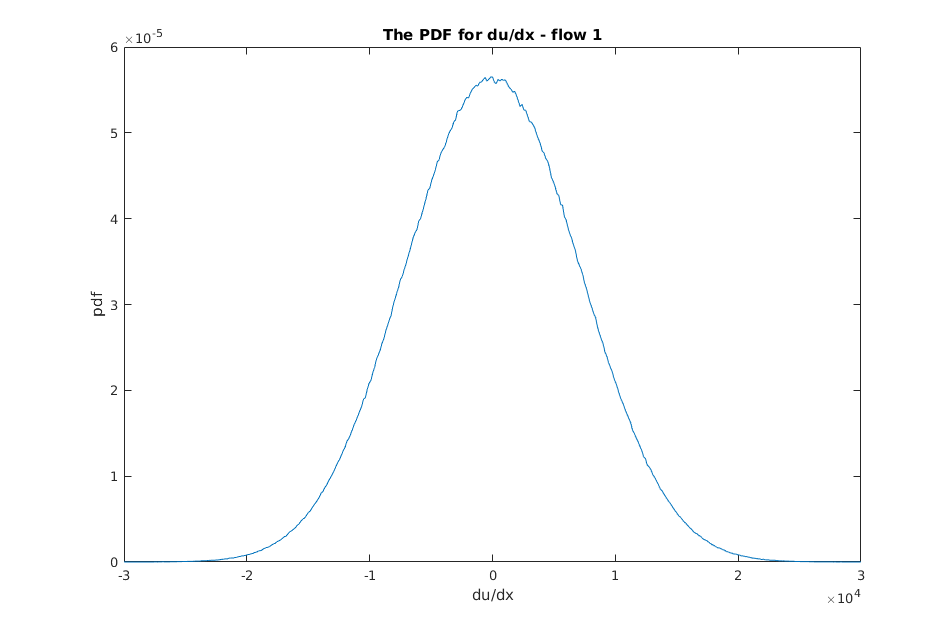
\includegraphics[scale=0.5]{./TEXT/dudx-pdf1.png}
\caption{The normalised Probability Density function of $^{\partial u_1} / _{\partial x_1}$ for \emph{flow 1}}
\label{dudx1}
\end{figure}

\begin{figure}[!ht]
\centering
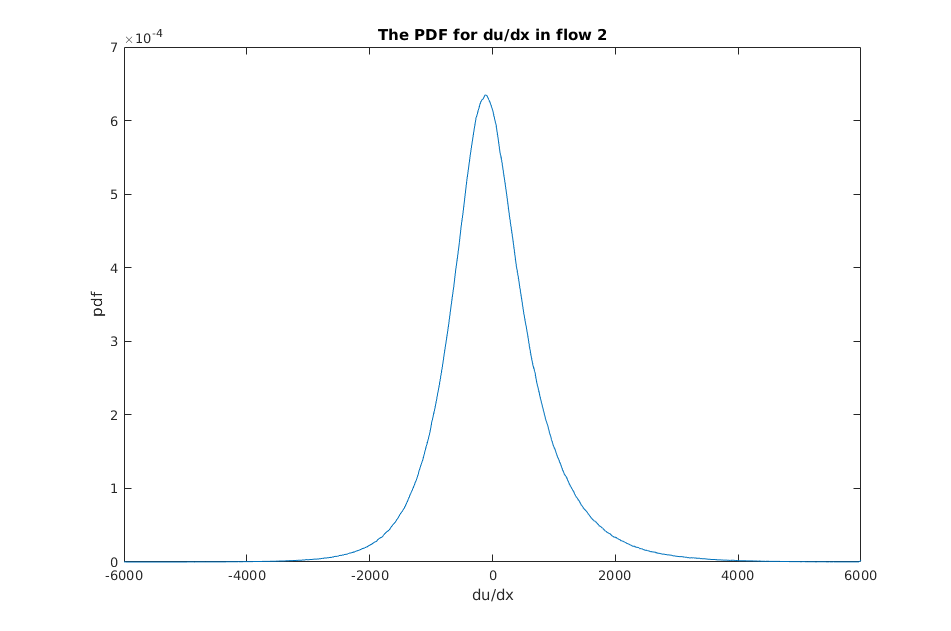
\includegraphics[scale=0.5]{./TEXT/dudx-pdf2.png}
\caption{The normalised Probability Density function of $^{\partial u_1} / _{\partial x_1}$ for \emph{flow 2}}
\label{dudx2}
\end{figure}

Figure \ref{dudx1} shows the probability distribution of $\partial u_1 / \partial x_1$ for \emph{flow 1}. The curve shows that the velocity derivative to be more evenly distributed for this flow than the second flow case (fig. \ref{dudx2}).

\emph{Kurtosis} is a measure of how 'spread out' a distribution is and it is often compared to the number $3$, given by the \emph{Gaussian} distribution. A kurtosis lower than this is said to be \emph{platykurtic} and a higher value is said to be \emph{leptokurtic}.
\emph{Skewness} shows if the data has more outliers towards the right (positive) or left end of the tails.

Table \ref{tbl2} shows that the high variance and low kurtosis suggest a more 'spread out' distribution for \emph{flow 1} when compared to the second. The second flow case is highly leptokurtic and the first is platykurtic but with a kurtosis close to that of a gaussian. The second case has more positive outliers due to the skewness of $0.55$ whereas in the first flow case the datapoints are well centered ($\emph{S} \approx 0$).

\begin{table}[ht]
\caption{Comparison of the first four moments for the $^{\partial u_1} / _{\partial x_1}$ of the two flows.}
\label{tbl2}
\centering
\begin{tabular}{l|c|c}
& Flow 1 & Flow 2 \\
\hline
1\su{st} Moment: Mean & $-0.002$ & $-0.225$\\
\hline
2\su{nd} Moment:Variance & $4.86 \times 10^7$ & $7.4 \times 10^{5}$\\
\hline
3\su{rd} Moment:Skewness & $-1.22 \times 10^{-4}$ & $0.55$\\
\hline
4\su{th} Moment:Kurtosis & $2.89$ & $5.92$\\
\hline
\end{tabular}
\end{table}